\documentclass[12pt,letterpaper]{article}

\usepackage{theusual}

\DeclareMathOperator*{\Var}{Var}

\def\f{\mathbf f}
\def\xx{{\bs{\xi}}}
\newcommand\ndots[1]{\mathrel{\overset{\makebox[0pt]{\mbox{\normalfont\tiny\sffamily $ #1$}}}{\cdots}}}
\def\N{{\mathcal N}}

\begin{document}

\hfill\textbf{\large Homework Assignment 4}

\hfill\textbf{Eugene Shvarts}

\hfill\textbf{ Stats 250 -- Baines -- Fall 2013 -- UC Davis}
\bigskip

\textbf{Problem \#1} \\ In this question, we implement a kernel to obtain samples from a truncated normal random variable, and test our code. \hrule \smallskip
\begin{enumerate}[a.]
\item Write a kernel in CUDA C to obtain samples from a truncated normal random variable of the form:
$$
X \sim TN\bigl(\mu,\sigma^2; (a,b)\bigr) \equiv N(\mu,\sigma^2) \1_{[a,b]}
$$
\textsf{Code attached.} \\ I used a naive rejection sampler with a tolerance of \texttt{maxnaive} attempts, and then switched over to the acception-rejection method detailed in Robert (2009) for at most \texttt{maxtries} attempts, after which I return \texttt{NA} in frustration. The method allows either or both truncation end point to be finite.

\item Compile your CUDA kernel using \texttt{nvcc} and check it can be launched properly.

I used the RCUDA instructions and (eventually) had no issues. My rng was initialized to $[1,2,3]$. Output was correctly returned, captured to file on \texttt{lipschitz}, and sent to my machine. I used \\
\texttt{.cuda(mykernel, out = x, n, mu, sigma, lo, hi, rnga, rngb, rngc, maxn, maxt, \\ gridDim = A\$grid\_dims, blockDim = A\$block\_dims, outputs = 'out')}

where $A$ is the output of the gridsize utility, and everything else is vectorized where necessary.

\item Sample 10,000 random variables from $TN(2,1;(0,1.5))$, and verify the expected value (roughly) matches the theoretical value.

The theoretical expected value, if $\phi$ is the standard normal and $\phi_{\mu,\sigma}$ is $\mathcal N (\mu,\sigma^2)$, is
$$
\frac{\int_A x\phi_{\mu,\sigma}}{\int_A \phi_{\mu,\sigma}} = \mu + \sigma \frac{\int_{A'} x\phi}{\int_{A'} \phi}~~,
$$
where $A$ is the original interval, and $A'$ is the interval with endpoints mapped through $x \mapsto (x-\mu)/\sigma$. For our parameters, Matlab computes an expected value of $0.9570066$. The simulated values from \texttt{rtruncnorm.cu} have mean $0.9513158$; one part in one hundred error looks like good agreement (obeying the square-root law, since we had ten thousand samples).

\item Write an R function for sampling truncated normal random variables, and sample 10,000 random variables from this function. Verify the mean (roughly) matches the theoretical values.

\textsf{Code attached.} \\ I tried several test runs; the samples produced consistently have a mean between $9.44$ and $9.60$. This is a good enough agreement for 10,000 samples.

\item Time the GPU and CPU code for a range of samples / iterations.

\begin{center}
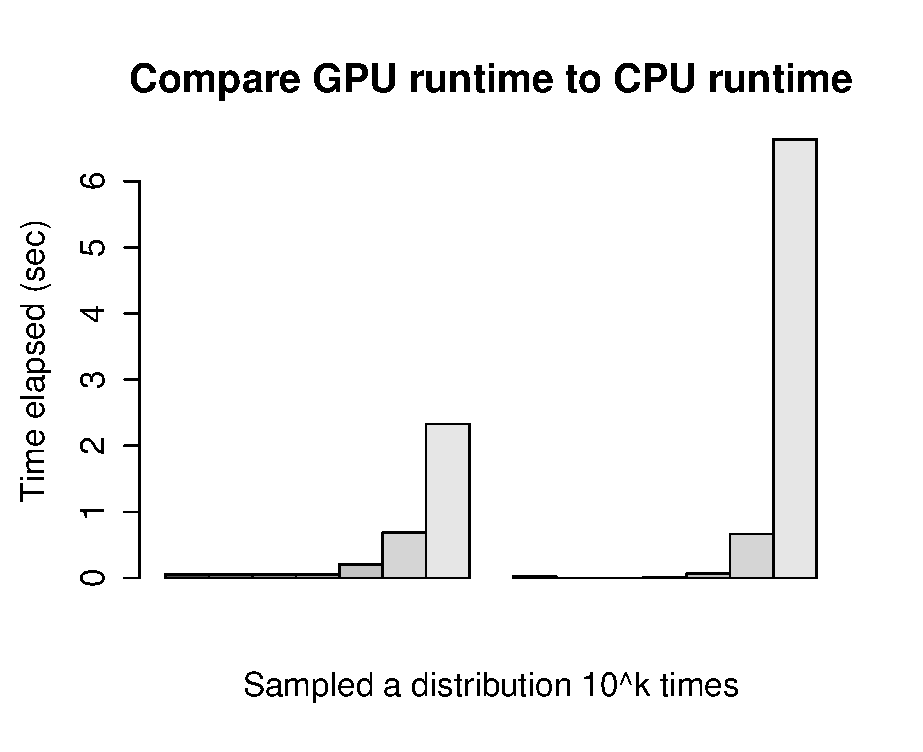
\includegraphics[height=8cm]{compare_GPU_CPU_time.eps}
\end{center}
I ran my CUDA (through RCUDA) and R code both on an AWS GPU instance, via the included \texttt{compute\_times.R}. I plotted the third component of the system time, i.e., the elapsed time. $10^8$ samples was too many for CUDA to handle via my code, but it's clear that the GPU will vastly outstrip the CPU at that order; on the order of $10^7$ samples (keeping in mind each is running potentially thousands of sub-computations in the accept-reject routine) they both take about $2$ seconds, and then the relative difference in computing time grows exponentially. 

\item , g. Verify that both codes work when $a$ and/or $b$ are infinite. Check an extreme region, e.g., $(\mu,\sigma,a,b) = (0,1,-\infty,-10)$. 

I took 10,000 samples from 3 different distributions using both GPU and CPU, and computed their means along with the actual expected value according to \texttt{quadgk} in Matlab. 

\begin{center}
\begin{tabular}{|c|c|c|c|}
\hline 
 & GPU mean & CPU mean & Expectation \\ 
\hline 
TN(4,4,-Inf,Inf) & 3.9648 & 4.0051 & 4.0000 \\ 
\hline 
TN(-1,2,0,Inf) & 1.2800 & 1.2717 & 1.2822 \\ 
\hline 
TN(0,1,-Inf,-10) & -10.0980 & -10.0984 & -10.0981 \\ 
\hline 
\end{tabular} 
\end{center}

\end{enumerate}
\smallskip

\textbf{Problem \#2} \\ In this question you will implement Probit MCMC i.e., fitting a Bayesian Probit regression model using MCMC. This model turns out to be computationally nice and simple, lending itself to a Gibbs sampling algorithm with each distribution available in sample-able form. The model is as follows:
\begin{align*} 
Y_i \sep Z_i &\sim \1_{Z_i>0} \\
Z_i \sep \beta &\sim \N(x_i^T \beta,1) \\
\beta &\sim \N(\beta_0,\Sigma_0)~~,
\end{align*}
where $\beta_0$ is a $p\times 1$ vector corresponding to the prior mean, and $\Sigma_0^{-1}$ is the prior precision matrix. \hrule \smallskip
\begin{enumerate}[a.]
\item , b. Write an R function \texttt{probit\_mcmc} to sample from the posterior distribution of $\beta$ using the CPU only. Then, modify the code so that all samples of $Z_i$ (i.e., all samples from a truncated normal) are performed by the GPU. 

\textsf{Code attached.} \\ Running \texttt{source(`probit\_mcmc')} loads RCUDA, all of the other relevant code I've made for the module, and your grid-size utility. $\beta$ is returned as an \texttt{mcmc} object, and both thinning and burn-in are available. 

\addtocounter{enumi}{1} \item Test both of your codes on the test file \texttt{mini\_data} generated via \texttt{sim\_probit} . 

While I can get my CPU regression code to work fine, and the stand-alone GPU-based sampler works like a charm, for some reason no matter how much I debug, it is absolutely impossible for me to combine the probit on CPU with sampling via GPU -- I repeatedly get a cornucopia of CUDA errors (CUDA\_ERROR\_LAUNCH\_FAILED , error launching CUDA kernel 400 , $\ldots$). I must be missing something simple; in any case my code is attached and on Github. 

\item Analyze as many of the large datasets generated by \texttt{sim\_probit} as you can, with both CPU and GPU code, and compare the run times. Use \texttt{niter = 2000, burnin = 500}. 

For the reasons mentioned above, I could only get CPU results (running on AWS, in this case). I ran

\texttt{system.time(\{ \\
a <- as.matrix(read.table('./data/data\_0i.txt',header=TRUE,sep=" ")); \\
probit\_mcmc(a[,-1],a[,1]) \} ) } with the asked-for parameters set as defaults, with $i = 1,2,3,4,\not{5}$. The results:

\begin{center}
\begin{tabular}{|c|c|c|c|c|}
\hline 
data\_01 & data\_02 & data\_03 & data\_04 & data\_05 \\ 
\hline 
00:16  & 02:36 & 23:22 & 3:50:00 & Loooong \\ 
\hline 
\end{tabular} 
\end{center}

I would've let the code run overnight, but I felt it was more prudent to turn it in. It would have been nice to do the GPU comparison; because the number of truncated-normal samples taken is $n + n \#_{mcmc} = O(n)$, so we should get roughly the same exponential (at least?) rate of improvement in the relative computation speed, where the CPU is outstripped within an order of magnitude or so of $n = 10^6$.


\end{enumerate}


\pagebreak
%\input{aux1-201c}

\end{document}